% MA-SQLGrid narrative revision, 2026-08-12. Numerical evidence is unchanged from the 2026-08-09 reference release.
\documentclass[applsci,article,submit,moreauthors]{Definitions/mdpi}
\firstpage{1}
\makeatletter\setcounter{page}{\@firstpage}\makeatother
\pubvolume{1}\issuenum{1}\articlenumber{0}\pubyear{2026}\copyrightyear{2026}
\datereceived{}\daterevised{}\dateaccepted{}\datepublished{}
\usepackage{booktabs}
\usepackage{algorithm}
\usepackage{algorithmic}
\setlength{\headheight}{20pt}
\setlength{\emergencystretch}{3em}
\newcommand{\masql}{MA-SQLGrid}
\AtBeginDocument{\pdfstringdefDisableCommands{\def\times{x}}}

\Title{MA-SQLGrid: A Robust and Auditable Multi-Agent Framework for Power-Grid Text-to-SQL}
\Author{Liu Bijing $^{1,2}$, Sun Chenglong $^{1,2}$ and Yang Yong $^{1,2,}$*}
\AuthorNames{Liu Bijing, Sun Chenglong and Yang Yong}
\address{$^{1}$ \quad NARI Group Corporation (State Grid Electric Power Research Institute), Nanjing 211106, Jiangsu Province, China;\\
$^{2}$ \quad Beijing Kedong Electric Power Control System Co., Ltd., Beijing 100080, China}
\corres{Correspondence: Yang Yong; liubijing@outlook.com}

\abstract{Power-grid databases encode asset, maintenance, status, temporal, and topological semantics that can make executable SQL answer the wrong question. We present \masql{}, a five-role architecture that organizes intent analysis, schema mapping, candidate normalization, read-only execution validation, and constructed-state evidence through a shared blackboard and deterministic controller. Robustness under tested conditions denotes mutation denial, bounded execution, and fail-closed handling of incomplete evidence. The evaluation combines GridDB generation, component, and constructed-state studies; BIRD Mini-Dev experiments across 11 public databases; and a fixed historical pool containing eight candidates for each of 180 GridDB questions. Context and presented-value effects depended on the frozen model snapshot. Within the historical pool, validation-aware ranking increased reference matches from 80/180 to 100/180, while complete three-witness evidence yielded 101/180. Both adjudicating selectors had top-score ties on 130/180 questions, and reversing candidate order produced 117--118/180, revealing that the available evidence often could not distinguish semantically competing candidates. \masql{} provides a practical and reproducible architecture for traceable power-grid Text-to-SQL research. The historical-pool comparison remains descriptive; unseen, expert-reviewed grid queries and budget-matched generation are required to establish broader efficacy.}
\keyword{text-to-SQL; multi-agent systems; power-grid databases; schema grounding; execution validation; constructed-state testing; reproducibility}
\featuredapplication{\masql{} is a research framework for traceable natural-language access to structured power-grid records. It exposes intent, schema, candidate, execution, and selection evidence so that generated SQL and returned rows can be inspected before consequential use.}

\begin{document}

\section{Introduction}

Power-grid organizations maintain relational data about assets, locations, topology, sensor readings, work orders, technicians, and maintenance activity. SQL provides precise access to these records, but it requires knowledge of table names, join keys, identifiers, units, aggregation conventions, and local coding rules. Text-to-SQL systems aim to reduce this access barrier by translating a natural-language request into an executable query. In an engineering workflow, however, a fluent query is not sufficient evidence of correctness. A query can execute while selecting the wrong status field, omitting a required filter, using an unintended join path, or returning the expected number of columns with the wrong content.

The risk is amplified by the semantics of grid records. An identifier that looks numeric may be a categorical code; a timestamp can refer to sensing, issuance, acknowledgement, or closure; and an asset status may describe the asset, an event, or a work order. The same request may therefore admit several executable queries with different engineering meanings. A useful workflow should expose how the request was interpreted, how schema and values were grounded, what SQL candidates were considered, which candidates executed, and why one candidate was selected. When the available evidence is incomplete, the workflow should be able to abstain rather than conceal the ambiguity.

Cross-database benchmarks such as Spider and BIRD have made schema generalization and realistic database content central evaluation concerns \cite{yu2018spider,li2023bird}. Spider~2.0 extends this setting to enterprise workflows with large schemas and multiple SQL dialects, while MultiSQL broadens context-dependent evaluation across diverse operations \cite{lei2025spider2,li2024multisql}. Schema-aware models, constrained decoding, context selection, decomposition, and execution guidance address complementary failure modes \cite{wang2020ratsql,scholak2021picard,nan2023enhancing,pourreza2023dinsql,talaei2024chess}. Recent systems also use multiple roles for generation, review, or repair \cite{lee2025team,wang2025macsql,shao2025qcmasql,xia2025r3}. Most studies optimize one or more of these stages, but fewer examine generation, database-enforced validation, state evidence, candidate selection, and trace retention as one reproducible decision process. This gap is important for grid data because an execution success alone provides weak evidence about field meaning, time scope, status coding, or join intent.

\masql{} addresses this systems problem through a five-role multi-agent architecture. The Query Analyst represents question intent; the Schema Cartographer maps that intent to tables, columns, values, and relationships; the SQL Synthesizer normalizes and identifies candidate statements; the Validation Engine records read-only execution evidence; and the Metamorphic-State Critic records outcomes on named constructed states. A deterministic controller coordinates these roles through a shared blackboard trace and either selects an eligible candidate or abstains. The controller is not a sixth reasoning agent. It enforces message order, evidence requirements, and the registered selection rule. This division makes errors localizable: a reviewer can determine whether a failure arose during intent analysis, schema mapping, candidate production, execution, state testing, or adjudication.

The empirical design examines this workflow from complementary angles. GridDB experiments vary schema context, structural hints, and presented values on a controlled power-grid schema. A constructed-state study examines whether observed results persist across registered database transformations. BIRD Mini-Dev tests the portability of frozen prompting procedures across 11 public, non-grid databases. Finally, a no-generation study applies fixed-order and evidence-aware selectors to the same historical pool of eight candidates per GridDB question. These studies do not form a single accuracy benchmark; together, they show where context, validation evidence, and deterministic selection affect observable behavior.

The study addresses three research questions:
\begin{enumerate}
\item How do schema context, value evidence, and prompting organization affect executable results for frozen models on GridDB and public databases?
\item When candidate generation is held fixed in a historical pool, how does evidence-aware adjudication change the selected query and its reference match relative to fixed order?
\item How stable are these observations across model snapshots, constructed database states, score ties, and candidate order?
\end{enumerate}

The paper makes three contributions. First, it presents \masql{}, a five-role framework that integrates intent analysis, schema mapping, candidate normalization, read-only execution validation, and state evidence in a traceable blackboard workflow. Second, it provides an evaluation design spanning GridDB, BIRD, constructed states, and a fixed historical candidate pool, allowing generation behavior, portability, validation behavior, and candidate selection to be observed separately. Third, it shows that validation-aware ranking increased reference matches from 80 to 100 of 180 questions within the historical pool, with complete witness evidence yielding 101 matches, while high tie rates and candidate-order sensitivity reveal a remaining semantic-ranking bottleneck.

In this paper, \emph{robustness under tested conditions} refers to mutation denial, bounded read-only execution, complete-evidence gating, and deterministic failure handling. The term \emph{multi-agent} denotes the five specialized roles and their coordinated trace. The present experiments do not estimate a causal five-role advantage over a call-matched single agent, and the historical-pool analysis remains descriptive. These scope conditions are revisited once in Section~5 rather than repeated for every result.

\section{Related Work}

\subsection{Schema Linking, Context Construction, and Evaluation}

Text-to-SQL systems map a natural-language request and database schema to an executable query. Spider established cross-domain evaluation on unseen databases, and BIRD expanded the setting toward larger databases with richer content \cite{yu2018spider,li2023bird}. Spider~2.0 and MultiSQL further emphasize enterprise-scale schemas, varied SQL operations, and context-dependent workflows \cite{lei2025spider2,li2024multisql}. These benchmarks make schema generalization visible, but their scores still depend on the database engine, evaluator, split, and model configuration.

Schema linking connects question spans to tables, columns, values, and foreign-key relations \cite{wang2020ratsql,lei2020reexamining,liu2022semantic}. Full-schema context protects recall but increases token cost and distraction. Compact context reduces the search space but can omit a bridge table or coded field. Retrieval, graph pathfinding, and bidirectional table--column selection seek a better balance \cite{bozdemir2026schema,liu2025solidsql,hao2025genlink,wang2025linkalign,safdarian2026schemagraphsql,nahid2026bidirectional}. Value examples add another signal because the intended field may be clearer from stored codes than from its name. The GridDB studies in this paper examine these context and value choices as observable components of a larger workflow.

Evaluation also needs more than one notion of match. String comparison can penalize equivalent SQL, while result equality can reward different queries that happen to coincide on one database snapshot. Test-suite accuracy and multiple database states reduce some accidental equivalence, provided that the state transformations preserve the intended relation. \masql{} therefore reports strict execution equality, constructed-state agreement, and bounded metamorphic invariance as distinct endpoints. Together they describe execution behavior; expert-reviewed business semantics remain a separate validation layer.

\subsection{Multi-Role Generation, Validation, and Selection}

Constrained decoding, decomposition, contextual grounding, and execution-guided repair address different stages of SQL production \cite{scholak2021picard,nan2023enhancing,sun2023sqlprompt,pourreza2023dinsql,talaei2024chess}. Recent workflows add question rewriting, attention-oriented decomposition, partition-and-drill reasoning, preference optimization, active database probing, or dialect-aware bootstrapping \cite{mao2024dartsql,xie2024deasql,luo2024ptdsql,zhai2025executionfeedback,xie2026sdesql,zhang2025exesql}. These methods mainly improve generation or repair. \masql{} focuses on the interfaces that connect candidate production to database-enforced validation and final selection.

SQL-oriented language-model teams distinguish candidate diversity from explicit role coordination \cite{lee2025team}. Multi-agent Text-to-SQL systems have used decomposition and tools, question-dependent routing, and review--rebuttal--revision consensus \cite{wang2025macsql,shao2025qcmasql,xia2025r3}. \masql{} assigns stable responsibilities to five roles and stores every handoff in a shared blackboard trace. The SQL Synthesizer may package candidates produced elsewhere, while the Validation Engine, Metamorphic-State Critic, and deterministic controller operate on explicit evidence. This design makes the trace, rather than only the final SQL, the unit of reproducibility.

Read-only execution and evidence-aware adjudication are complementary. Database controls prevent an admissible evaluation from mutating the source, whereas adjudication compares only candidates that satisfy the required safety, execution, and state-evidence gates. A stored trace cannot guarantee sound reasoning, but it can reveal whether an error entered through intent analysis, schema mapping, generation, execution, or selection. This diagnostic role motivates the framework even when candidate generation is held fixed.

\subsection{Power-Grid Text-to-SQL}

Power-system data combine topology, equipment attributes, measurements, time series, costs, constraints, and maintenance records. RTS-GMLC and SimBench provide reproducible engineering structures that can be transformed into relational databases \cite{barrows2020rts,meinecke2020simbench}. Their availability does not by itself produce an expert-reviewed Text-to-SQL benchmark: intended projections, units, ordering, tie handling, and time semantics still require domain adjudication.

DKA-SQL is a direct power-grid Text-to-SQL precedent that adapts domain knowledge to grid questions \cite{bian2025dkasql}. Its corpus and evaluation boundary differ from the present study. \masql{} instead investigates a systems architecture for traceable role coordination, read-only validation, constructed-state evidence, and deterministic candidate selection. GridDB supplies a controlled grid case study, BIRD supplies public cross-database portability evidence, and RTS-GMLC/SimBench assets identify a path toward broader structural validation. Table~\ref{tab:literature-position} summarizes this positioning without treating results from different datasets and call budgets as directly comparable.

\begin{table}[htbp]
\caption{Positioning against adjacent Text-to-SQL approaches; entries describe reported design emphasis, not comparable performance.}
\label{tab:literature-position}\centering\small
\resizebox{\textwidth}{!}{%
\begin{tabular}{p{0.20\textwidth}p{0.22\textwidth}p{0.22\textwidth}p{0.26\textwidth}}
\toprule
Approach & Principal emphasis & Evaluation setting & Difference from \masql{}\\
\midrule
RGISQL \cite{li2024rgisql} & Grammatical and relational graph modeling & Public Text-to-SQL tasks & Learned generator rather than a traced executor/adjudicator boundary\\
Zero-shot prompting \cite{zhou2025zeroshot} & Prompt strategies and LLM behavior & Public benchmarks & Prompt comparison without the five-role blackboard\\
Schema retrieval \cite{bozdemir2026schema} & Embedding/vector-store context selection & LLM SQL generation & Retrieval quality rather than fail-closed named-state selection\\
DKA-SQL \cite{bian2025dkasql} & Domain knowledge adaptation & Power-grid Text-to-SQL & Different corpus and implementation; not reproduced here\\
\masql{} & Five-role trace, read-only validation, state evidence, and deterministic selection & GridDB case study plus BIRD portability & Integrates generation-to-selection evidence for power-grid Text-to-SQL\\
\bottomrule
\end{tabular}
}
\end{table}

\section{Materials and Methods}

\subsection{Problem Formulation and System Overview}

For question $x_i$, read-only database $D_i$, and introspected schema $S_i$, a generator produces one or more candidates
\begin{equation}
\mathcal{Y}_i=\{\widetilde{y}_{i1},\ldots,\widetilde{y}_{ik}\}.
\end{equation}
Each candidate must satisfy a single-statement read-only contract. The accepted leading form is \texttt{SELECT} or \texttt{WITH}; comments, multiple statements, write operations, schema changes, attachments, and pragmas are rejected. A candidate is eligible for adjudication only when it is safe and executable.

The offline evaluator may later compare the selected query with a reference result. Let $E_i=1$ when the selected SQL executes and its result equals the frozen reference result under the registered evaluator, and $E_i=0$ otherwise. Reference SQL, reference results, $E_i$, and any derivative correctness field are forbidden from all five agents and the Adjudicator. Evaluation occurs only after the blackboard is sealed.

This boundary yields three distinct objects. A candidate is \emph{admissible} when its syntax and requested operations satisfy policy, \emph{executable} when it completes within the registered database limits, and \emph{correct under the frozen evaluator} when its result matches the reference after sealing. Admissibility is neither executability nor correctness. The manuscript preserves all three labels because collapsing them would let an executable but semantically wrong query appear validated.

The framework's response contract contains the selected SQL, stable candidate and source identifiers, referenced tables and columns, execution-state and result hashes, state-coverage summary, abstention or selection reason, and the sealed trace digest. Figure~\ref{fig:coordination} shows how these records move through the five-role multi-agent architecture. The controller is not a sixth reasoning model: it schedules the roles, checks their typed messages, applies the deterministic rule, and seals the shared blackboard trace before offline evaluation.

\begin{figure}[htbp]
\centering
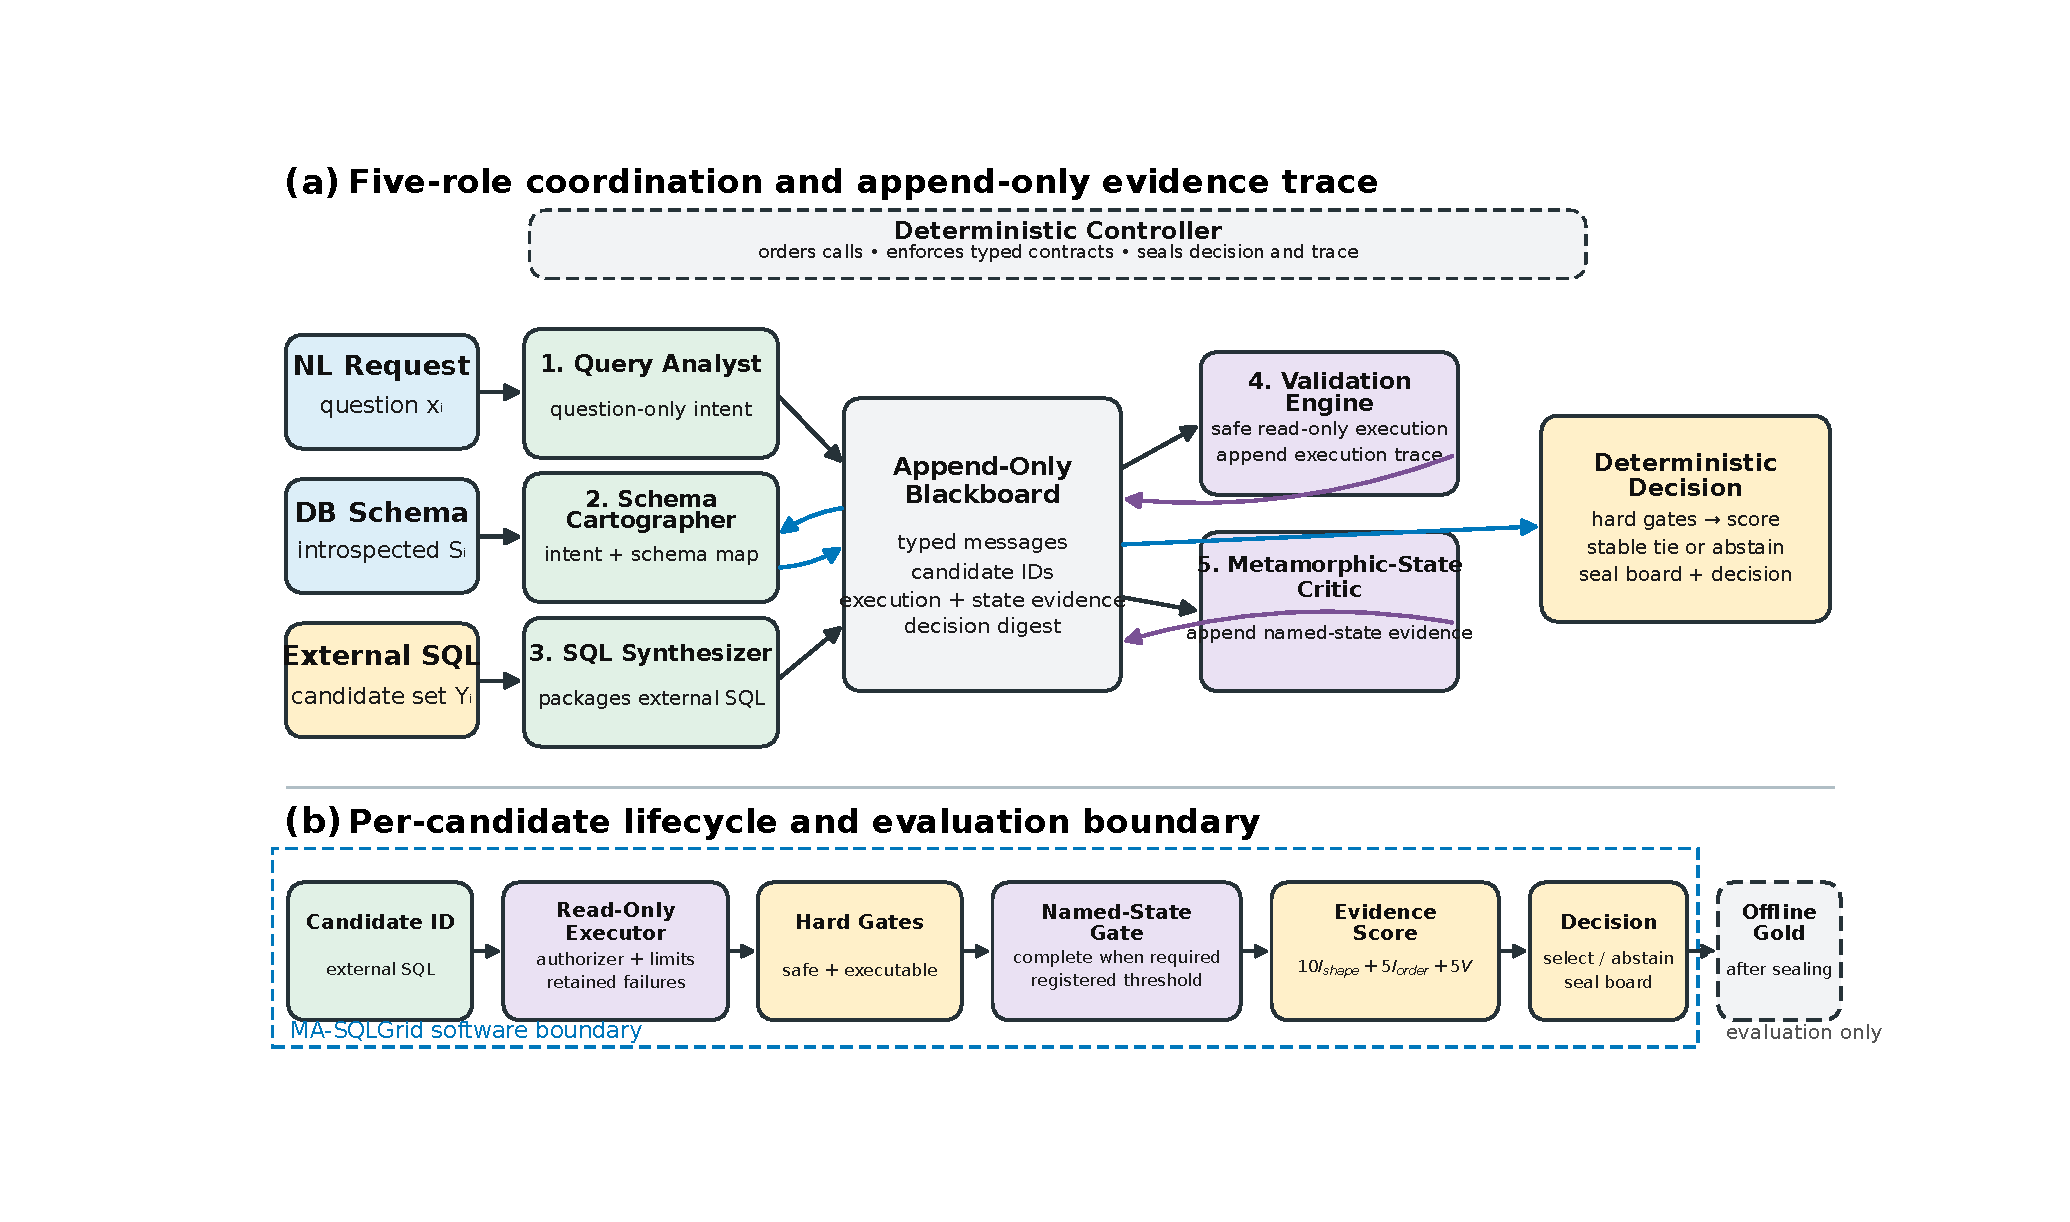
\includegraphics[width=0.98\textwidth]{figures/fig_ma_sqlgrid_dual_panel.pdf}
\caption{\masql{} information flow and candidate lifecycle. \textbf{(a)} The Query Analyst and Schema Cartographer post question and schema records to the shared blackboard, and the SQL Synthesizer normalizes externally supplied candidates. The Validation Engine records read-only execution evidence, while the Metamorphic-State Critic records named-state evidence when required. \textbf{(b)} Hard eligibility gates precede the effective evidence score $e(y)=10I_{\mathrm{shape}}+5I_{\mathrm{order}}+5V$, $V\in[0,1]$, and the deterministic tie or abstention rule. Reference results are loaded only after the decision and trace digest are sealed.}
\label{fig:coordination}
\end{figure}

The response contract supports traceability rather than user authorization. A calling application must authenticate the user, restrict the accessible database view, and decide whether returned rows may be displayed. Generated SQL and execution success do not replace those institutional controls.

\subsection{Datasets and Evaluation Roles}

GridDB-Maintenance-v2 v0.1 is a synthetic SQLite case study with eight tables and 98 rows: \texttt{asset\_types} (6), \texttt{assets} (18), \texttt{grid\_topology} (9), \texttt{locations} (8), \texttt{maintenance\_logs} (8), \texttt{sensor\_readings} (26), \texttt{technicians} (8), and \texttt{work\_orders} (15). It contains 200 natural-language--SQL records: 20 development records and 180 factorial evaluation records. The evaluation records include 66 easy, 91 medium, and 23 hard items and map to 70 normalized gold-SQL structural clusters, of which 58 are singletons. The evaluation partition had been visible during project development; it is a controlled finite-set case study, not a sealed production benchmark.

BIRD Mini-Dev contributes 500 public items over 11 SQLite databases. The protocol froze order, prompts, two local models, evaluator, Python 3.10.11/SQLite 3.40.1, and zero retries. Each backbone made 2500 calls and produced 2000 final predictions; independent re-execution found zero score mismatches. Two earlier failed attempts totaling 2476 calls remain immutable excluded incidents.

The GridDB reliability release contains 18 states: the canonical snapshot, three insertion permutations, and 14 additional schema-valid stress states. The scorer produced 25,920 prediction-state rows ($1440\times18$). A prediction-blinded automated protocol admitted a 66-question subset for the primary 15-state analysis and retained 114 order-sensitive questions as diagnostics. These constructed states are not operator-certified grid snapshots.

Four provenance labels distinguish the evaluation inputs. Inherited records predate this manuscript revision; Recomputed results are deterministic transformations of retained inputs; New records were generated under a protocol frozen before outcome access; and Diagnostic records test implementation behavior. The coordination-core replay is Diagnostic because it verifies handoffs and deterministic execution rather than SQL accuracy.

Evidence classes preserve chronology: Inherited predictions and outcomes predate the framework; Recomputed processes retained inputs without new generation; New requires inputs, rules, and visibility to be frozen before outcome access; and Diagnostic permits post hoc inspection only. Labels apply per result because the manuscript contains several classes.

Table~\ref{tab:resources} separates the resources by domain and evaluation role. GridDB supports controlled generation, component, state, and historical-pool analyses. BIRD tests portability across public non-grid databases. RTS-GMLC and SimBench provide authentic power-system structures, but their current question--SQL pairs remain machine-generated silver resources because qualified-human semantic review has not been completed.

\begin{table}[htbp]
\caption{Data-resource scope and evidence status. Counts describe retained local artifacts; they are not interchangeable benchmark denominators.}
\label{tab:resources}
\centering
\small
\setlength{\tabcolsep}{3pt}
\resizebox{\textwidth}{!}{%
\begin{tabular}{p{2.2cm}rrrrp{2.4cm}p{3.0cm}}
\toprule
Resource & DBs & Tables & Rows & NL--SQL & Evidence class & Visibility and review status\\
\midrule
GridDB v0.1 & 1 & 8 & 98 & 200 & Synthetic grid; inherited development case & 20 dev + 180 evaluation; development-visible; no documented independent dual-expert review\\
GridDB state suite & 18 states & 8 & state-dependent & 0 new & Constructed grid-state diagnostic & Prediction-blinded state construction; not operator-certified\\
RTS-GMLC pilot & 1 & 10 & 360,530 & 55 & Authentic grid structure; machine silver & \texttt{AUTO\_CANDIDATE}; 0 human-reviewed; 0 sealed; source-use notice applies\\
SimBench pilot & 1 & 8 & 874 & 36 & Authentic grid structure; machine silver & Development-visible; 0 human-reviewed; 0 sealed; ODbL/DbCL review required before redistribution\\
BIRD Mini-Dev & 11 & dataset-specific & dataset-specific & 500 & Public non-grid portability benchmark & Frozen public split; BIRD v1.1 protocol; not evidence of power-grid validity\\
\bottomrule
\end{tabular}}
\end{table}

\subsection{Experimental Protocols and Evaluation Boundaries}

Table~\ref{tab:protocol-master} maps each protocol to its unit, endpoint, and evidence boundary. The studies answer complementary questions and are interpreted separately because their candidate sources, call budgets, and visibility histories differ.

\begin{table}[htbp]
\caption{Experimental design, estimand, and inferential role of each protocol. Composition intervals describe sensitivity to the observed finite-corpus grouping and are not population confidence intervals.}
\label{tab:protocol-master}\centering\scriptsize
\begin{tabular}{p{1.9cm}p{1.85cm}p{2.3cm}p{2.45cm}p{3.0cm}}
\toprule
Study & Unit/groups & Generation design & Endpoint/inference & Research role\\
\midrule
GridDB factorial & 180 questions/cell; 70 normalized-SQL groups & one call per item and cell & execution equality; finite-corpus contrasts with nine-test Holm correction & context and hint effects for two frozen model snapshots\\
Component E1/E2 & 170 paired or 180 questions; 61 or 70 groups & 700 calls under a frozen procedure & execution equality; grouped composition intervals and registered families & value-evidence and multi-candidate-selection effects\\
Constructed states & 66 primary questions; 12 structural groups & no new generation calls & 15-state logical AND; exact $2^{12}$ signs with nine-test Holm correction & agreement under prediction-blind database transformations\\
BIRD v1.1 & 500 items; 11 databases & one call for B0--B2 and two for B3 & execution accuracy; database-grouped intervals and 12 Holm-adjusted contrasts & public non-grid cross-database portability\\
Coordination replay & 180 questions; no grouping & no new generation calls & pool coverage; complete finite-pool counts & trace and handoff reproducibility\\
Historical-pool selection & 180 questions; no grouping & common ledger of 5760 attempts & reference match after board sealing; rescue/harm, ties, and order sensitivity & deterministic evidence-aware selection within the observed pool\\
\bottomrule
\end{tabular}
\end{table}

GridDB factorial outcomes are inherited and development-visible; the component call-and-selection procedure was frozen before calls on development-visible items; formal-v5 states were constructed without reading predictions; and BIRD used a frozen public protocol. The historical-pool study sealed every decision before directly loading raw reference outcomes, but same-item derived outcomes had been accessed earlier in the development history. Its selector comparisons are consequently descriptive, even though their execution is deterministic and traceable.

\subsection{Five-Role Multi-Agent Architecture}

\masql{} comprises five specialist roles coordinated by the controller shown in Figure~\ref{fig:coordination}. Messages receive consecutive sequence numbers, and the complete trace is serialized canonically to a SHA-256 digest. Each role has a restricted input and produces one typed output for the next stage.

The \textbf{Query Analyst} produces a structured question-only intent record containing lexical tokens, detected aggregations, ordering requirements, and an explicit limit when present. It does not select SQL or see correctness. The \textbf{Schema Cartographer} maps lexical intent to tables, columns, and foreign-key edges. The current skeleton uses deterministic overlap and records unmatched tokens; a richer GridDB adapter adds disclosed domain rules and graph expansion.

The \textbf{SQL Synthesizer} packages external SQL without model calls, canonicalizes formatting, removes exact duplicates while preserving first occurrence, and assigns stable identifiers. The release-v3 \textbf{Validation Engine} opens a frozen database using \texttt{mode=ro\&immutable=1}, enables \texttt{query\_only}, disables extensions, and installs an authorizer. It denies writes, DDL, transactions, attachments, pragmas, metadata enumeration, dangerous functions, and reads outside table/column allowlists; progress and fetch handlers enforce time, opcode, and row limits. Every attempt retains database/SQL hashes, failures, timing, row count, and result hash without hidden retry.

The later FINAL executor adds function allowlisting, projected-width, raw-cell-byte, and total-result-byte limits. Fourteen tests cover 1/5/50 MB BLOB denial, total-budget and exact-boundary behavior, trace retention, oversized text/results, and wide projections. These controls were not used for the v3 ledger or 80/100/101 counts. Table/column allowlists constrain query scope but do not authenticate users or provide row-level authorization; both variants establish tested SQLite mutation denial and scoped execution bounds, not data minimization, process isolation, or operational approval.

The threat model assumes untrusted SQL but a trusted host, SQLite library, configured allowlist, and immutable database. It does not address a compromised process, OS escape, side channels, built-in malicious extensions, or upstream authorization errors. Production use requires process isolation, least-privilege views, authenticated context, logging, and independent security review.

Failure handling is intentionally fail-closed and non-retrying. A parse denial, authorizer denial, timeout, opcode limit, row limit, width limit, cell limit, or total-result limit creates a retained attempt record and makes that candidate ineligible for the current decision. The controller cannot silently weaken a limit or substitute a repaired query. A repair procedure may be studied as a separate registered generation step, as in BIRD B3, but its extra physical call and visibility must remain explicit.

The \textbf{Metamorphic-State Critic} (the historically named Counterfactual Critic) consumes named state results, rejects duplicate state identifiers, and records evaluated, passed, failed, and missing states. When state evidence is optional, missing evidence remains diagnostic and does not break prior no-state behavior. When the caller requires state evidence, coverage must equal the complete registered state set and the pass threshold must be met; otherwise the candidate is ineligible. Thus an incomplete 1/1 record cannot outrank a complete 10/11 record. Existing formal-v5 labels compare predictions with gold and remain forbidden during selection.

The blackboard is append-only at the application layer: a role posts a typed message and cannot rewrite an earlier message. The controller checks role, message type, sequence number, and required fields before acceptance. Canonical serialization fixes key order and whitespace before hashing. This makes two runs comparable at the trace level and exposes an unexpected hidden field or changed handoff. It does not prevent a malicious host process from altering memory or files; process isolation and remote attestation are outside scope.

Information flow is intentionally asymmetric. The Analyst receives the question but no candidate SQL. The Cartographer receives the question, intent record, and introspected schema. The Synthesizer receives external candidate strings and assigns identities but cannot execute them. The Validator receives one candidate plus a scoped executor. The Critic receives named-state outcomes but no reference correctness. Only the deterministic Adjudicator receives the eligible evidence summaries. Gold enters a separate offline evaluator after the decision message and board digest exist.

\subsection{Read-Only Validation and Evidence-Aware Adjudication}

Eligibility always requires safety and successful execution. The archived 100-point representation assigns 40 points for each of those two properties, followed by 10 for question-derived aggregate-shape conformity, 5 for question-derived ordering conformity, and up to 5 for lexical value hits. Because every ranked candidate has already passed both hard gates, the first 80 points are constant and contain no ranking information. The effective evidence score is therefore $e(y)=10I_{\mathrm{shape}}(y)+5I_{\mathrm{order}}(y)+5V(y)$ for an eligible candidate $y$, with $V(y)\in[0,1]$. When named-state evidence is optional, the controller selects an $\arg\max e(y)$ and ties preserve frozen candidate order. When named-state evidence is required, incomplete coverage or failure of the registered pass threshold makes $y$ ineligible before the same ranking. If the eligible set is empty, the controller abstains. This piecewise gate--score--tie function is mathematically equivalent to the archived implementation; it exposes that safety/execution are eligibility controls rather than discriminative score evidence. V3 does not establish that the weight design preceded access to derived outcomes for the 180 items, so weight, pass-threshold, and reversed-order results remain descriptive sensitivity analyses.

The archived 40/40/10/5/5 allocation---equivalently, hard safety/execution gates followed by a 10/5/5 evidence score---is an illustrative deterministic policy, not a learned, calibrated, or theoretically optimal weighting and not an algorithmic performance contribution. Its formal invariants are: an unsafe or non-executable candidate is never selected; required named-state coverage is complete before its threshold is evaluated; gold-derived correctness is absent from the decision record; equal scores resolve by the frozen order; and an empty eligible set yields abstention. These invariants support conformance testing and replay determinism. They do not imply semantic correctness, calibrated confidence, or superiority over a simpler policy.

Question-derived shape checks are deliberately weak. They detect cues such as ``how many'', ``highest'', ``first'', and explicit limits and compare them with the projected aggregate or ordering structure. They do not infer business semantics such as whether ``active'' refers to an asset, alarm, or work-order state. Lexical value hits likewise reward only presented values traceable to the question and context; they are not evidence that the associated column is the intended one. These low-bandwidth features keep adjudication inspectable but explain why large tie sets remain possible.

Abstention has two layers. Pre-ranking abstention occurs when no candidate passes safety and execution requirements or when required state coverage is incomplete. Post-ranking ambiguity is currently resolved by stable order rather than abstention because no pre-registered margin threshold exists in v3. The high tie rates observed later show that future work should freeze an ambiguity policy---for example, abstaining on unresolved top ties or requesting a user clarification---before examining new outcomes.

Robustness under tested conditions is represented by four observable mechanisms: database mutation denial, bounded execution, complete named-state eligibility, and deterministic failure handling. Candidate-order stability is assessed separately in Results. Algorithm~\ref{alg:coordination} states the resulting reference-isolated coordination rule.

\begin{algorithm}[htbp]
\caption{Reference-isolated deterministic coordination}
\label{alg:coordination}
\begin{algorithmic}[1]
\REQUIRE question $x_i$, schema $S_i$, external candidates $\mathcal{Y}_i$, read-only executor, named state evidence
\STATE post structured intent and schema grounding to the append-only blackboard
\STATE canonicalize and deduplicate externally produced candidates
\FOR{each candidate $y\in\mathcal{Y}_i$}
  \STATE apply single-statement read-only validation
  \STATE record execution and available reference-free state evidence
\ENDFOR
\IF{required named-state coverage is incomplete for a candidate}
  \STATE mark that candidate ineligible (fail closed)
\ENDIF
\IF{no safe executable candidate meets all registered gates}
  \STATE abstain
\ELSE
  \STATE apply the fixed validation, state-evidence, coverage, and order rule
\ENDIF
\STATE post the decision and seal the blackboard
\STATE load reference results only for offline evaluation
\end{algorithmic}
\end{algorithm}

\subsection{Generation Study}

The paired design crosses context package $c\in\{0,1\}$ and composite hint $h\in\{0,1\}$. F00 uses full DDL and global values without the hint; F01 adds the hint; F10 uses compact domain-grounded context without the hint; and F11 combines compact context and the hint. The same 180 questions appear in all four cells for each backbone, yielding 720 Qwen and 720 Granite predictions.

Because each question appears in every prompt cell, cell differences are paired within question. The two backbone snapshots form parallel finite-corpus experiments rather than independent replications drawn from a model population. Difficulty labels and normalized-SQL clusters are retained as descriptive structure. Cluster-based randomization reduces the influence of near-duplicate SQL forms, while composition-sensitivity intervals show how estimates vary when observed clusters are resampled. Neither procedure converts this development-visible synthetic set into a population sample.

Qwen2.5-Coder-7B Q4\_K\_M and Granite-3.3-8B Q4\_K\_M were run at temperature zero with fixed snapshots. Each prompt produced exactly one response. The parser retained the first SQL candidate through the first semicolon; the validator then applied the read-only policy. There was no candidate ranking, multi-agent negotiation, or repair in this experiment.

Strict execution equality is primary. A common-target projected-column indicator is a secondary manipulation check. Paired finite-set contrasts use normalized-SQL clusters as dependence proxies, registered sign-flip tests, composition-sensitivity bootstrap intervals, and Holm correction. The intervals describe sensitivity to the observed corpus composition, not population confidence.

\subsection{Component, Constructed-State, and Public-Database Studies}

The separately frozen component study contains 700 scored calls. E1 compares candidate generation with and without presented value evidence on 170 paired questions in 61 frozen groups. E2 requests up to three candidates and compares a deterministic reference-answer-independent selector with the first candidate on 180 questions in 70 groups. Question-level paired differences are averaged with equal question weights; bootstrap resampling and sign assignments operate at group level. Selection is sealed before gold loading. Rescue, harm, and oracle-at-three are descriptive; oracle-at-three is a gold-only upper-bound diagnostic. The three two-member Holm families are E1 across backbones, E2 across backbones, and the two cross-backbone modifiers.

The v5 reliability protocol reproduced all 1440 T0 labels and then executed every prediction over 18 states. The primary 66-question analysis uses a question-weighted logical-AND endpoint over 15 semantic states. A prediction passes only when it agrees with the reference on every included state. The nine registered contrasts form a separate Holm family; with only 12 structural groups, all $2^{12}=4096$ group-sign assignments are enumerated. The sharp-null interpretation assumes exchangeability of those 12 group signs; the small group count limits randomization resolution, and the groups are dependence proxies rather than sampled deployment clusters.

The BIRD protocol compares direct prompting, decomposition, schema selection, and bounded execution repair. Each method has a fixed call pattern and zero retries. Accuracy and method differences retain equal item weighting over 500 items; pairwise randomization assigns one common sign to all paired item differences within each of 11 databases and applies Holm correction across 12 comparisons. Its sharp-null interpretation assumes database-level sign exchangeability. Eleven clusters give coarse attainable evidence and do not represent a random sample of power-grid databases.

The four protocols answer different questions and are not pooled. GridDB factorial cells test prompt-package manipulations on a controlled grid schema. E1 and E2 test presented values and reference-independent selection. Formal-v5 tests agreement across constructed states, and BIRD tests non-grid workflow portability.

\subsection{Historical-Pool Selection Study}

The replay verifies SHA-256 for two 720-row prediction ledgers and the 25,920-row formal-v5 ledger before reading them. For each question it pools the eight existing outputs from two backbones and four prompt cells, canonicalizes SQL, and removes duplicates. Frozen T0 fields provide execution and metadata-shape evidence. The Critic records named-state evidence as unavailable because existing state-agreement labels are gold-relative.

This is a coverage diagnostic. Candidates were generated under different models and prompt packages; the pool is not a deployable, matched multi-agent run. No selected output is compared with gold to produce an accuracy number.

The release-v3 study reuses exactly eight frozen source slots for each of the 180 GridDB evaluation questions: four Qwen prompt cells followed by four Granite prompt cells. It performs no LLM call and creates no new question or SQL label. Before any method selects, the three methods share one precomputed eight-by-four execution ledger: T0 plus three metamorphic witnesses for every slot. Thus 5760 is the shared physical evidence-collection count, not a separate natural runtime cost assigned to each selector. The fixed-order control ignores the collected ranking evidence and chooses slot 0. Validation-only ranks candidates without named-state evidence, whereas complete-witness selection requires all three reference-free metamorphic outcomes. Incomplete coverage or no passing candidate causes abstention.

The three query-blind witnesses have distinct SHA-256 values and are built from T0 without reading questions, prompts, predictions, scores, or gold. M1 adds an irrelevant relation and rows; M2 adds harmless indexes and rebuilds storage; M3 adds nullable probe columns to three business tables. M1 and M2 preserve original-schema denotation. M3 preserves explicitly projected original columns but deliberately allows wildcard projection to fail. Query order is preserved when candidate SQL contains \texttt{ORDER BY}; otherwise rows are compared as a multiset. The selector sees only question text extracted from frozen prompt ledgers, the schema, eight SQL strings, executor traces, and T0-to-witness equivalence. It does not see gold SQL, answer-shape metadata, correctness, difficulty, feature tags, required literals, or gold-relative formal-v5 labels.

These witnesses test metamorphic relations rather than alternative ground-truth answers. M1 asks whether an irrelevant table changes behavior, M2 whether logically neutral storage changes alter the result, and M3 whether projection is stable when nullable columns are appended. A pass means that the observed result satisfies the registered relation; it does not mean the original query expresses the user's intent. A fail can reveal brittleness, as with wildcard projection, but may also reflect a transformation outside the intended query equivalence class. For this reason, witness outcomes enter eligibility only under the disclosed construction and remain reference-free diagnostics.

Candidate order is a first-class experimental variable because the adjudicator uses stable order for equal scores. Original order places four Qwen slots before four Granite slots and follows the prompt-cell sequence within each backbone. Reverse-order sensitivity changes only this tie breaker after the same evidence has been collected. It is therefore a direct diagnostic of unresolved ranking information, not an alternative model or a new sample. The large change later observed under reversal motivates an abstention or clarification policy for future work.

Each selector inherited the same 1440 source slots and 5760 attempts, and no failed candidate was replaced or retried. The complete software-test matrix, version chronology, manifest hashes, and excluded predecessor records are provided in Supplementary Sections S1--S3. These records establish the provenance of the historical pool; they do not change its descriptive status.

Descriptive endpoints are strict execution accuracy over all 180 questions, coverage and abstention, complete-three-witness invariance of the selected candidate, and rescue/harm relative to fixed order. The retained sensitivity matrix crosses three weight policies, invariant-pass thresholds of 1/3, 2/3, and 3/3 while always requiring complete observation, and original versus reversed candidate-order tie breaking. Because same-item outcomes were accessible before v3, this matrix is reported only as descriptive analysis.

\subsection{Statistical Analysis}

The statistical unit is the question, and every question receives equal weight. The principal estimand is the mean paired difference on the observed finite corpus. Normalized-SQL groups for GridDB and databases for BIRD are dependence proxies used for grouped resampling and sign assignment; they are not random samples from a deployment population. Composition-sensitivity intervals describe how a finite-corpus estimate changes when the observed groups are reweighted and are not population confidence intervals.

The randomization procedures assume exchangeability of group-level signs under the tested sharp null. Exact enumeration is used for the 12-group constructed-state analysis ($2^{12}=4096$ assignments), while the larger registered families use the retained Monte Carlo procedures and seeds. All tests are two-sided, zero paired differences are retained in the estimand and contribute no sign, and the Holm families are defined separately for the nine GridDB factorial effects, projected-column manipulation checks, three two-member component families, nine constructed-state contrasts, and 12 BIRD pairings. Count differences, paired effects, rescue/harm, and sensitivity results remain visible whether or not a Holm-adjusted decision is met.

The historical-pool comparison is reported through complete counts, paired rescue/harm, coverage, abstention, tie multiplicity, and candidate-order sensitivity. Because same-item outcomes were accessible during earlier development, these quantities describe the frozen pool and do not support a population or causal multi-agent effect.

\subsection{Implementation and Reproducibility}

The local generation experiments used the identified Qwen2.5-Coder-7B-Instruct Q4\_K\_M and Granite-3.3-8B-Instruct Q4\_K\_M snapshots under frozen protocols. The BIRD formal protocol fixed Python 3.10.11, SQLite 3.40.1, model order, prompts, evaluator, and zero retries. The five-role controller, read-only executor, state-evidence gate, and deterministic replay have regression and adversarial tests. Main-text results always retain the control version actually used to generate them; later executor corrections are reported as implementation evidence and are not applied retroactively.

Detailed version records, artifact hashes, test inventories, incident histories, rights information, and release validation are placed in the Supplementary Materials. This separation keeps the main text focused on the research design while preserving computational provenance for editors and reviewers.

\subsubsection{Generative-AI Assistance and Author Responsibility}

The local SQL-generation experiments used the explicitly identified Qwen2.5-Coder-7B-Instruct Q4\_K\_M and Granite-3.3-8B-Instruct Q4\_K\_M snapshots under the frozen protocols described above. Separately, during reconstruction and revision of this manuscript, the authors used the OpenAI Codex agent interface to propose and edit prose, suggest experimental and audit checks, review and draft Python/\LaTeX{} code, assemble provenance and response matrices, and assist local build and visual-quality checks. The exact backend model identifier and version for every Codex session were not retained in the project records; this provenance boundary is reported explicitly, and no unrecorded model identifier is inferred.

All executable suggestions were run locally against retained inputs, and reported numerical results were taken from frozen or independently recomputed ledgers rather than accepted from generated prose. The authors retained responsibility for protocol authorization, evidence-class decisions, interpretation, citations, declarations, and the final manuscript. Codex output was not treated as qualified power-system expert annotation or adjudication. External machine-generated question--SQL candidates remain labeled machine silver and do not become human gold through model review. All six scientific figures are deterministic code-native graphics with file-level lineage; no generative-image model supplied quantitative evidence.

\section{Results}

\subsection{Overview of Empirical Findings}

The experiments produced three main observations. First, schema context, structural hints, and presented values affected the two frozen model snapshots differently; no single context strategy dominated across every analysis. Second, evidence-aware adjudication changed the selected candidate within the frozen historical pool: reference matches increased from 80/180 under fixed order to 100/180 under validation ranking and 101/180 with complete witness evidence. Third, both adjudicating selectors produced top-score ties on 130/180 questions, and reversing candidate order yielded 117--118/180 matches. Validation evidence therefore helped reject some weaker candidates, but the available semantic signals often remained too coarse for stable ranking.

The following subsections separate these findings by research question. GridDB and BIRD results address context and portability; the historical-pool analysis addresses evidence-aware selection; and the constructed-state, tie, and order analyses address stability. Implementation conformance is summarized after the empirical results and documented fully in the Supplementary Materials.

\subsection{Context and Component Effects on SQL Generation}

All 1440 scheduled predictions are present, and independent SQLite re-execution reproduced the stored execution verdicts. Table~\ref{tab:cells} reports strict execution equality, and Figure~\ref{fig:cells} visualizes the same audited cell estimates.

\begin{table}[htbp]
\caption{Strict execution equality over 180 GridDB questions per cell.}
\label{tab:cells}
\centering
\small
\setlength{\tabcolsep}{4pt}
\begin{tabular}{lcccc}
\toprule
Backbone & F00 full/no hint & F01 full/hint & F10 compact/no hint & F11 compact/hint\\
\midrule
Qwen & 76/180 (0.4222) & 129/180 (0.7167) & 78/180 (0.4333) & 108/180 (0.6000)\\
Granite & 77/180 (0.4278) & 100/180 (0.5556) & 74/180 (0.4111) & 108/180 (0.6000)\\
\bottomrule
\end{tabular}
\end{table}

\begin{figure}[htbp]
\centering
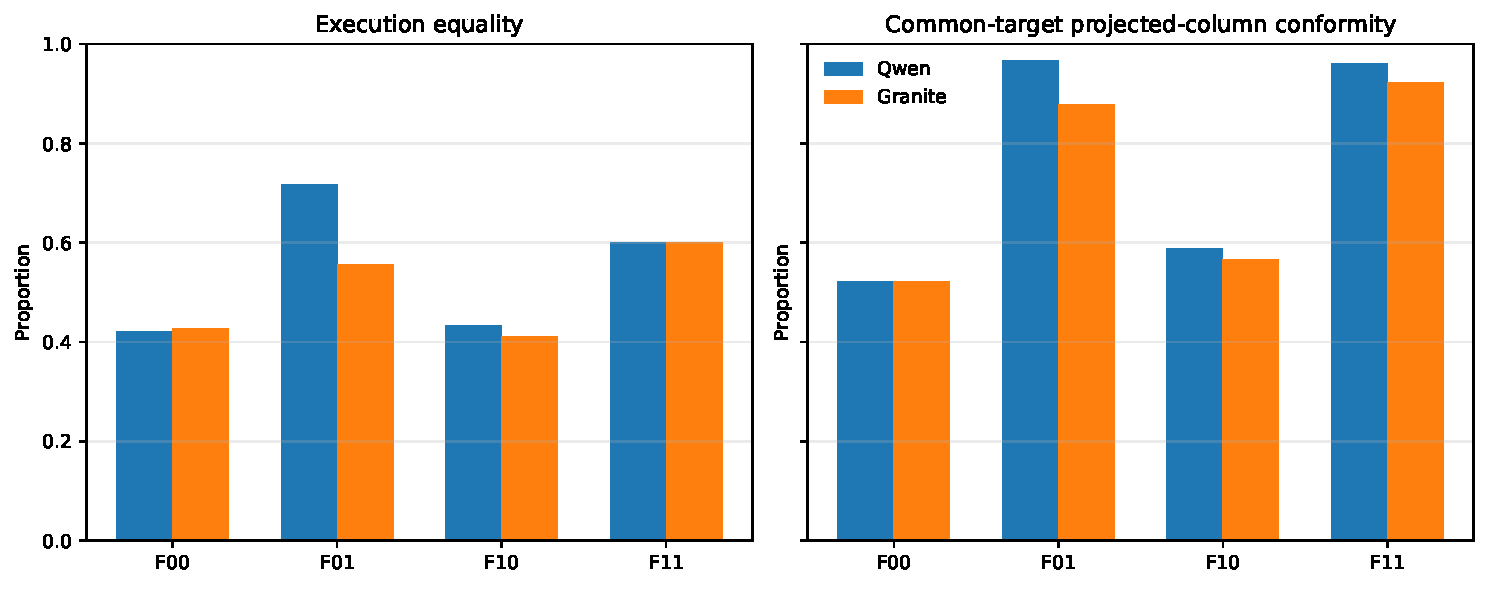
\includegraphics[width=0.94\textwidth]{figures/results/fig01_v2_cells.pdf}
\caption{Audited GridDB cell point estimates. Each cell contains all 180 attempts; the figure is descriptive and does not replace registered factorial contrasts.}
\label{fig:cells}
\end{figure}

The common-target projected-column diagnostic is 0.5222 in F00 for both backbones. Qwen obtains 0.9667, 0.5889, and 0.9611 in F01, F10, and F11; Granite obtains 0.8778, 0.5667, and 0.9222. Returning the requested number of columns is therefore easier than returning the intended rows. In Qwen F01, projected-column conformity is 0.9667 while execution equality is 0.7167.

The eight cells also show why a single best prompt cannot represent the design. Adding the hint to full context increases the point estimate for both backbones, whereas adding compact context without the hint leaves execution equality close to F00. Under compact context, the hint produces 108 correct answers for both models, but this numerical convergence arises from different unhinted baselines and does not establish identical behavior. Complete cell reporting preserves these interactions rather than selecting only the highest cell.

The 0.2500 gap between Qwen F01 projected-column conformity and strict execution equality warns against structural proxy endpoints. A model may recognize that one column, an aggregate, or an ordered row is requested while still choosing the wrong table, join, predicate, value, or boundary. Shape diagnostics can localize errors and inform adjudication, but they cannot replace result equality or qualified semantic review.

\subsubsection{Factorial Effects and Multiplicity}

Table~\ref{tab:factorial-nine} reports the complete primary family. For Qwen, the composite-hint execution effect is +0.2306, the package--hint interaction is $-0.1278$, and the compact-package main effect is $-0.0528$. Granite's corresponding estimates are +0.1583, +0.0611, and +0.0139. Zero of nine primary execution tests survives Holm correction. Qwen's hint effect has raw/adjusted $p=0.01372/0.09604$, its interaction $0.00919/0.07352$, and the cross-backbone hint modifier $0.00640/0.05760$. No primary factorial execution effect or modifier is therefore described as statistically nonzero.

\begin{table}[htbp]
\caption{Complete primary factorial family for strict execution equality. Estimates are question-weighted finite-set differences; intervals are 95\% normalized-SQL-group composition-sensitivity intervals. Each sign-randomization used 70 groups, 100,000 draws, and the displayed raw values were Holm-adjusted jointly over all nine rows.}
\label{tab:factorial-nine}\centering\scriptsize
\resizebox{\textwidth}{!}{%
\begin{tabular}{llrrrr}
\toprule
Scope & Effect & Estimate & Composition interval & Raw $p$ & Holm $p$\\
\midrule
Qwen & Compact-package main & -0.0528 & [-0.1131, 0.0000] & 0.10523 & 0.52614\\
Qwen & Structural-hint main & 0.2306 & [0.0548, 0.4355] & 0.01372 & 0.09604\\
Qwen & Package $\times$ hint & -0.1278 & [-0.2454, -0.0341] & 0.00919 & 0.07352\\
Granite & Compact-package main & 0.0139 & [-0.0584, 0.0798] & 0.85021 & 1.00000\\
Granite & Structural-hint main & 0.1583 & [-0.0193, 0.3662] & 0.15480 & 0.61919\\
Granite & Package $\times$ hint & 0.0611 & [-0.0539, 0.2013] & 0.55890 & 1.00000\\
Granite--Qwen & Backbone $\times$ package & 0.0667 & [-0.0360, 0.1814] & 0.41478 & 1.00000\\
Granite--Qwen & Backbone $\times$ hint & -0.0722 & [-0.1229, -0.0276] & 0.00640 & 0.05760\\
Granite--Qwen & Three-way interaction & 0.1889 & [0.0090, 0.4321] & 0.07010 & 0.42060\\
\bottomrule
\end{tabular}}
\end{table}

The normalized-SQL mapping contains 70 groups, 58 singletons, and a maximum group size of 19. Question-level weighting is retained; groups are resampling and sign-assignment proxies, not verified authoring templates or sampled clusters. The randomization interpretation requires exchangeability of group signs under the tested sharp null, while the composition interval asks how the finite-corpus mean changes when those observed groups are reweighted. Neither assumption follows from the data, and the high singleton fraction limits protection against unmeasured dependence.

The displayed composition intervals are pointwise sensitivity intervals; they are neither simultaneous/familywise intervals nor inversions of the nine Holm-adjusted randomization tests. An interval that excludes zero can therefore coexist with a Holm non-rejection. The multiplicity decision, not interval exclusion, controls statements about the registered nine-test family.

No minimum practically important execution-accuracy difference, equivalence margin, or non-inferiority margin was registered. Therefore the study cannot infer practical equivalence from a non-rejection, and the 1/180 complete-witness difference is only a mechanism trace rather than a meaningful-benefit result.

In the separately corrected secondary family, the common-target hint effects survive: +0.4083 for Qwen (adjusted $p=0.000090$) and +0.3556 for Granite (adjusted $p=0.01944$). Because the hint supplies structural information later scored by this endpoint, these are manipulation-check results, not independent semantic evidence.

The multiplicity result changes the emphasis of the factorial study. Large raw contrasts motivate hypotheses about structural instructions, but none of the nine primary execution comparisons meets the registered familywise rule. The projected-column findings verify that the manipulation changed a closely aligned surface property. They do not show that the compact package or hint produces a backbone-independent accuracy gain. Future work should separate schema pruning, value presentation, normalization, and structural hints rather than retaining composite packages.

\subsubsection{Presented Values and Candidate Selection Components}

The component run completed all 700 scored calls under a prospectively frozen call-and-selection procedure on development-visible GridDB items. On the paired 170-question subset, Qwen first-candidate correctness changed from 83/170 to 101/170, a +0.1059 difference (95\% composition-sensitivity interval [+0.0282, +0.2013], adjusted $p=0.0310$). Granite remained 69/170 in both paired conditions, with an interval spanning zero. The cross-backbone modifier did not meet the registered rule, so the Qwen result is not replicated across backbones and is not a five-role result.

The deterministic selector changed 24 Qwen and 36 Granite choices. Relative to the first candidate, it rescued eight and harmed one Qwen question, and rescued ten while harming none for Granite. Execution effects were +0.0389 and +0.0556; neither survived its two-test Holm family. Oracle-at-three values of 0.6389 and 0.4667 are gold-only diagnostics and are not deployable selector results.

For Qwen, the value-evidence intervention adds 18 correct first candidates when the 170 eligible V0 questions are compared with their V1 counterparts under the registered analysis; the corresponding Granite estimate is zero. The disagreement is more informative than averaging the backbones: the effect depends on how a frozen model uses schema and value context. Oracle-at-three measures candidate-pool headroom, whereas the reference-free selector measures how much of that headroom the recorded rule can recover without gold.

Complete component counts are retained in the numerical supplement. On all 180 V1 questions, Qwen first/selector/oracle-at-three counts were 105/112/115, and Granite counts were 71/81/84; the paired 170-question intervention counts and all registered effects appear in Table~\ref{tab:component-effects}. These are component, not five-role, outcomes.

\begin{table}[htbp]
\caption{Complete component-effect families. Intervals are pointwise group-composition sensitivity summaries, not simultaneous intervals and not inversions of the Holm tests. Each family contains the two displayed members indicated by its identifier.}
\label{tab:component-effects}\centering\scriptsize
\resizebox{\textwidth}{!}{%
\begin{tabular}{llrrrrrr}
\toprule
Family & Contrast & $N$ & Groups & Estimate & Composition interval & Raw $p$ & Holm $p$\\
\midrule
E1 & Qwen V1--V0 first candidate & 170 & 61 & 0.1059 & [0.0282, 0.2013] & 0.01552 & 0.03104\\
E1 & Granite V1--V0 first candidate & 170 & 61 & 0.0000 & [-0.1902, 0.1705] & 1.00000 & 1.00000\\
E2 & Qwen selector--first V1 & 180 & 70 & 0.0389 & [-0.0081, 0.1071] & 0.50080 & 0.50080\\
E2 & Granite selector--first V1 & 180 & 70 & 0.0556 & [0.0075, 0.1232] & 0.06425 & 0.12850\\
Cross-E & Granite--Qwen E1 effects & 170 & 61 & -0.1059 & [-0.2701, 0.0394] & 0.26986 & 0.53971\\
Cross-E & Granite--Qwen E2 effects & 180 & 70 & 0.0167 & [-0.0062, 0.0457] & 0.37477 & 0.53971\\
\bottomrule
\end{tabular}}
\end{table}

The three retained two-member Holm families are E1 across backbones, E2 across backbones, and Cross-E across modifiers. The Granite E2 pointwise interval excludes zero while its adjusted decision does not meet the registered rule; these summaries are not contradictory. The 61- and 70-group mappings retain question weights but are dependence proxies rather than a probability sample. Figure~\ref{fig:components} visualizes these effects without replacing the adjusted decisions.

\begin{figure}[htbp]
\centering
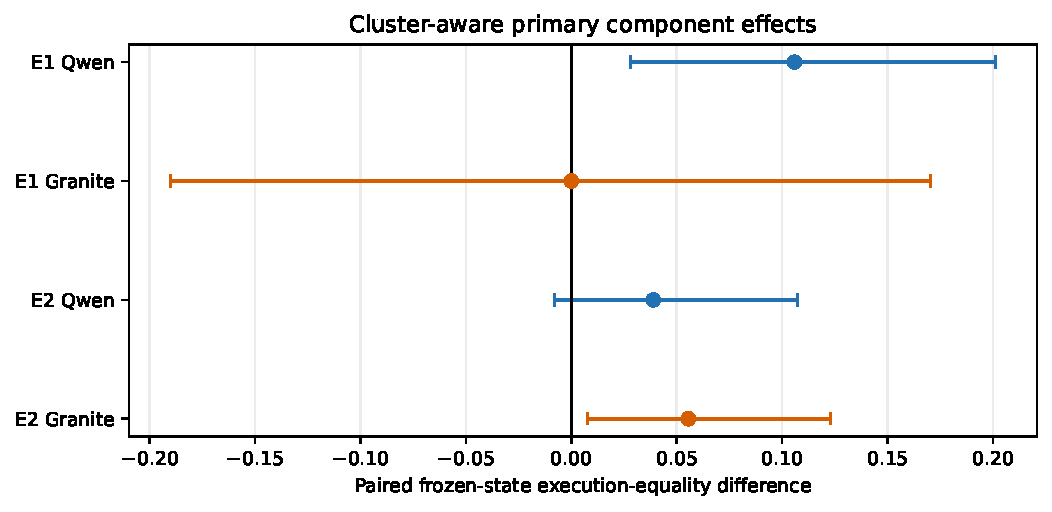
\includegraphics[width=0.92\textwidth]{figures/results/figure_01_primary_effects.pdf}
\caption{Component effects under a prospectively frozen call-and-selection procedure on development-visible GridDB items. Intervals describe composition sensitivity; the registered decision also requires multiplicity-adjusted evidence.}
\label{fig:components}
\end{figure}

\subsection{Constructed-State Stability}

The v5 scorer produced all 25,920 registered rows, and its T0 slice reproduced 1440/1440 snapshot labels. Table~\ref{tab:multistatecounts} and Figure~\ref{fig:multistate} report the 66-question automatic subset: 15-state logical-AND rates range from 0.6212 (Granite F01) to 0.8182 (Granite F00). All nine Holm-adjusted values equal 1.0000 under exact cluster-sign enumeration. No context, hint, interaction, or cross-backbone multi-state effect meets the declared rule. These rates characterize constructed-state agreement, not population accuracy or human-certified equivalence.

The ordering under this endpoint differs from the single-snapshot table. Granite F00 has the highest logical-AND rate on the 66-question automatic subset even though Granite F11 has the larger T0 execution count over all 180 questions. The denominators and endpoints differ, so this is not a contradiction. It demonstrates why a robustness statement must name both the admitted question subset and the required state set.

\begin{table}[htbp]
\caption{Complete 15-state logical-AND counts for the prediction-blinded 66-question automatic subset.}
\label{tab:multistatecounts}
\centering
\small
\begin{tabular}{lcccc}
\toprule
Backbone & F00 & F01 & F10 & F11\\
\midrule
Qwen & 49/66 (0.7424) & 48/66 (0.7273) & 53/66 (0.8030) & 43/66 (0.6515)\\
Granite & 54/66 (0.8182) & 41/66 (0.6212) & 51/66 (0.7727) & 49/66 (0.7424)\\
\bottomrule
\end{tabular}
\end{table}

\begin{figure}[htbp]
\centering

\includegraphics[width=0.92\textwidth]{figures/results/fig04_semantic_reliability.pdf}
\caption{GridDB multi-state logical-AND agreement for the prediction-blinded automatic subset. The endpoint is a constructed-state robustness diagnostic.}
\label{fig:multistate}
\end{figure}

\subsection{Cross-Database Portability on BIRD}

Table~\ref{tab:bird} reports all eight cells. BIRD Mini-Dev is a public non-grid portability benchmark and does not validate power-grid semantics. B0--B2 use one physical generation call per item; B3 uses two, so the inherited comparison estimates frozen workflow efficacy under unequal call counts rather than a call-matched repair effect. Each backbone completed 2500 calls, 2000 final predictions, zero retries, and zero final-ledger omissions; latency and token totals were not promoted into the retained summary and are therefore reported as unavailable rather than reconstructed.

\begin{table}[htbp]
\caption{Inherited BIRD Mini-Dev v1.1 results (non-grid portability evidence; 11 database clusters). Intervals are database-cluster composition-sensitivity intervals.}
\label{tab:bird}
\centering
\small
\setlength{\tabcolsep}{3pt}
\begin{tabular}{llrrrrp{1.5cm}}
\toprule
Backbone & Method & Correct/500 & Accuracy & Interval & Calls/item & Final-ledger omissions\\
\midrule
Qwen & B0 direct & 189/500 & 0.378 & [0.286, 0.470] & 1 & 0\\
Qwen & B1 decomposition & 151/500 & 0.302 & [0.203, 0.401] & 1 & 0\\
Qwen & B2 schema selection & 197/500 & 0.394 & [0.279, 0.511] & 1 & 0\\
\cmidrule(lr){1-7}
Qwen & B3 execution repair & 174/500 & 0.348 & [0.250, 0.452] & 2 & 0\\
Granite & B0 direct & 102/500 & 0.204 & [0.125, 0.284] & 1 & 0\\
Granite & B1 decomposition & 105/500 & 0.210 & [0.131, 0.294] & 1 & 0\\
Granite & B2 schema selection & 101/500 & 0.202 & [0.137, 0.273] & 1 & 0\\
\cmidrule(lr){1-7}
Granite & B3 execution repair & 118/500 & 0.236 & [0.159, 0.318] & 2 & 0\\
\bottomrule
\end{tabular}
\end{table}

After Holm adjustment, Qwen decomposition is 0.076 below direct prompting (adjusted $p=0.0430$), and schema selection is 0.092 above decomposition (adjusted $p=0.0117$). No Granite contrast survives correction. Different method orders across the two model snapshots argue against a universal prompting recipe. The two failed incident runs totaling 2476 physical calls remain excluded and immutable; they are not retries contributing to these denominators.

The BIRD results also constrain the meaning of ``agentic'' improvement. Decomposition reduces Qwen accuracy relative to direct prompting, while bounded repair uses twice the physical calls without becoming the best Qwen method. Granite shows a different descriptive ordering and no adjusted contrast. More stages or calls therefore do not guarantee a better outcome. A future comparison must count physical generations, retries, context tokens, and failed attempts, not only final predictions.

\subsection{Validation-Aware Selection in the Historical Candidate Pool}

The replay audited all 180 GridDB questions without a generation call. At least two distinct frozen SQL candidates were present for 173 questions. After safety checks and binding to consistent T0 execution evidence, 172 questions had at least two eligible candidates and entered retrospective adjudication. Seven failed closed because only one unique SQL remained, and one failed because fewer than two candidates were eligible.

Of 180 audited questions, 173 had at least two unique frozen SQL candidates and 172 retained at least two eligible candidates for retrospective adjudication; seven failed closed with one unique candidate and one with fewer than two eligible candidates. No reference-free named-state evidence was available. Unique-candidate multiplicities from one through eight occurred for 7, 19, 15, 18, 27, 23, 45, and 26 questions, respectively. These counts establish interface coverage, not correctness, execution gain, rescue, or multi-agent superiority.

\subsubsection{Reference Matches, Coverage, and Rescue/Harm}

The deterministic descriptive re-execution retained 5760 candidate--state attempts; 332 were non-executable or authorization/resource/SQL failures and remained in the all-attempt ledger. Every question nevertheless had at least one eligible candidate, so both adjudicating selectors covered 180/180 questions and abstained on 0/180. This zero-abstention result is a consequence of at least one eligible slot plus forced stable-order resolution of post-ranking ties, not confidence-calibrated coverage. Table~\ref{tab:offline} reports the recorded rules.

Keeping all 332 failures matters for two reasons. Removing them would overstate the executability of the historical pool, and retaining their slot identities verifies that selectors did not receive replacements or retries. Full question-level coverage means only that another slot was eligible for every question; it does not mean every candidate was valid or that an operational system should always answer.

\begin{table}[htbp]
\caption{Descriptive release-v3 re-execution over one historical eight-slot pool per question. All methods choose after the same precomputed candidate/evidence ledger of 32 attempts per question. Accuracy is finite-corpus strict execution equality after all blackboards were sealed; this is not a new-generation or five-role end-to-end experiment.}
\label{tab:offline}
\centering
\small
\resizebox{\textwidth}{!}{%
\begin{tabular}{lrrrrrr}
\toprule
Selector & Correct/180 & Accuracy & Covered & Abstained & Invariant & Rescue/harm\\
\midrule
Fixed order, shared ledger & 80/180 & 0.4444 & 180 & 0 & 177/180 & 0/0\\
Validation rank, shared ledger, no CF & 100/180 & 0.5556 & 180 & 0 & 179/180 & 22/2\\
Complete-three-witness selector & 101/180 & 0.5611 & 180 & 0 & 180/180 & 23/2\\
\bottomrule
\end{tabular}}
\end{table}

Figure~\ref{fig:offline-diagnostics} juxtaposes the two recorded endpoints. Validation-only and complete-witness selection differ by one frozen-reference match and one invariant selection. This small incremental change contrasts with their 20--21-match difference from fixed order and focuses interpretation on validation ranking and tie policy rather than on a broad counterfactual benefit.

\begin{figure}[htbp]
\centering
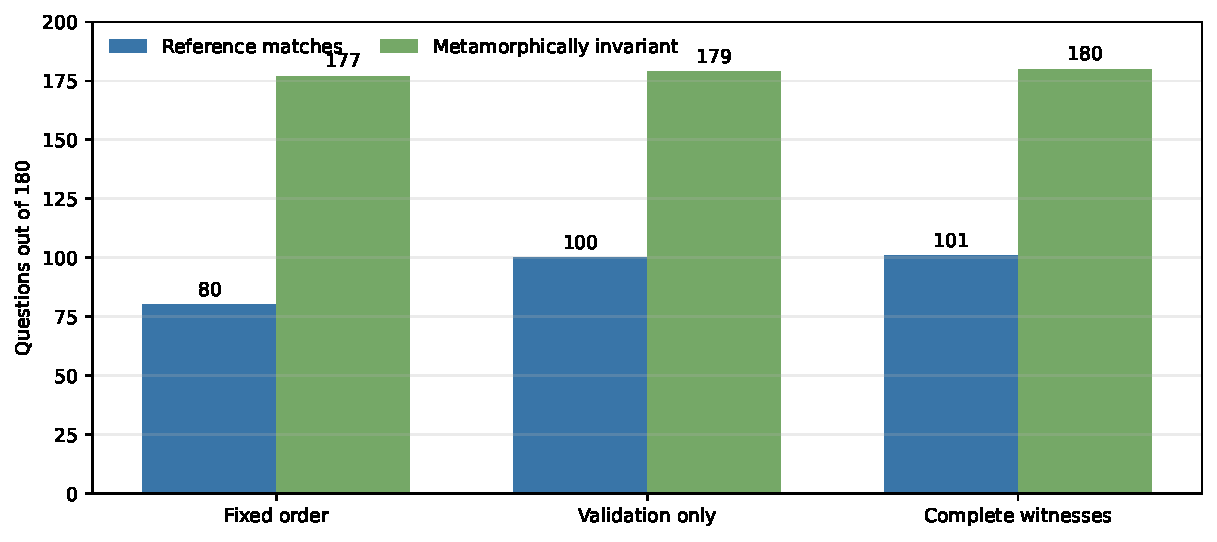
\includegraphics[width=0.90\textwidth]{figures/fig05_offline_selector_diagnostics.pdf}
\caption{Descriptive release-v3 selector endpoints over 180 historical-pool questions. Reference matches are loaded only after board sealing; invariance denotes agreement across the three constructed witnesses. Bars are not a prospective multi-agent comparison.}
\label{fig:offline-diagnostics}
\end{figure}

The two adjudicating selectors each had multiple highest-scoring candidates on 130/180 questions. Mean top-tie sizes were 5.4000 and 5.3889; all eight candidates tied on 79 validation-only and 78 complete-witness questions. With original-order tie breaking, 178/180 selections came from Qwen slots, reflecting source order rather than learned preference.

Thus, most apparent source preference is mechanically induced. When all eight candidates tie, the first slot is selected regardless of backbone quality; when seven tie, the earliest surviving slot has the same advantage. The observed 178 Qwen selections measure how often the available reference-independent features failed to separate candidates before the stable-order rule acted, rather than a learned preference for one backbone.

The complete multiplicity and selected-slot distributions are retained in the numerical supplement. Validation-only tie-size counts for sizes 1--8 were 50/5/3/4/5/8/26/79; complete-witness counts were 50/5/3/4/5/9/26/78.

Validation-only ranking added 20 net reference matches relative to fixed order through 22 rescues and 2 harms. Complete-witness selection changed the chosen candidate on only Q039, yielding one further match (101/180 versus 100/180), one additional rescue, no additional harm, and no coverage or abstention change. Table~\ref{tab:q039} gives the constructed trace for this sole difference.

\subsection{Tie Structure, Order Sensitivity, and the Q039 Case}

\begin{table}[htbp]
\caption{Q039 is the sole validation-only versus complete-witness selection difference. Correctness is agreement with the frozen synthetic reference, not an independently adjudicated engineering judgment.}
\label{tab:q039}
\centering
\footnotesize
\resizebox{\textwidth}{!}{%
\begin{tabular}{p{2.5cm}p{4.6cm}p{4.6cm}p{2.2cm}}
\toprule
Field & Validation-only & Complete witnesses & Interpretation\\
\midrule
Natural-language request & \multicolumn{2}{p{9.2cm}}{``Show the first scheduled work order after June 2024.''} & Ambiguous: ``after June'' can imply after 30 June, and ``scheduled'' can denote a status or merely a scheduled date.\\
Selected query & \texttt{SELECT * FROM work\_orders WHERE scheduled\_date > '2024-06-01' ORDER BY scheduled\_date ASC LIMIT 1} & \texttt{SELECT work\_order\_id, scheduled\_date FROM work\_orders WHERE scheduled\_date > '2024-06-01' ORDER BY scheduled\_date ASC LIMIT 1} & Both omit an explicit scheduled-status predicate and use a date boundary whose intended meaning lacks expert adjudication.\\
M3 outcome & Fails when nullable columns extend wildcard width & Preserves the explicit two-column projection & Constructed projection-stability behavior\\
Frozen-reference match & Incorrect & Correct & Outcome-exposed 1/180 trace only\\
\bottomrule
\end{tabular}}
\end{table}

M3 added nullable columns to \texttt{work\_orders}; consequently, complete-witness eligibility rejected the wildcard projection and retained the explicit \texttt{work\_order\_id, scheduled\_date} projection. The case shows how a constructed state can expose projection brittleness. Neither query resolves the request's status and date-boundary ambiguity through qualified review, so the extra reference match is interpreted as a projection-stability trace rather than an engineering correctness judgment.

Table~\ref{tab:sensitivity} reports all 18 sensitivity cells. Every original-order cell produced 101/180; reverse order produced 117/180 under default and intent-emphasis weights and 118/180 under validation-equal weights. These more favorable values are outcome-exposed diagnostics, not preferred alternatives. The 16--17-item shift and high tie multiplicity show that the apparent selector behavior is materially order-dependent.

Threshold invariance across 1/3, 2/3, and 3/3 occurs because the selected candidates' recorded witness patterns and score ties do not change the final original-order choices under these policies. The reverse-order increase cannot justify changing the frozen policy after observing outcomes. Instead, the 16--17-item shift diagnoses inadequate discriminative evidence and motivates a pre-registered tie or abstention rule for the next pool.

\begin{table}[htbp]
\caption{Complete-witness selector sensitivity summarized across invariant-pass thresholds. Results were identical at 1/3, 2/3, and 3/3 for every weight/order pair; coverage was 180/180 throughout.}
\label{tab:sensitivity}
\centering
\small
\resizebox{\textwidth}{!}{%
\begin{tabular}{lrrr}
\toprule
Weight policy & Thresholds represented & Original order correct/180 & Reverse order correct/180\\
\midrule
Default & 1/3, 2/3, 3/3 & 101 (0.5611) & 117 (0.6500)\\
Intent emphasis & 1/3, 2/3, 3/3 & 101 (0.5611) & 117 (0.6500)\\
Validation equal & 1/3, 2/3, 3/3 & 101 (0.5611) & 118 (0.6556)\\
\bottomrule
\end{tabular}}
\end{table}

The numerical supplement contains all eight GridDB cells, 12 component endpoints, eight 15-state cells, 18 sensitivity cells, the 360-row item-level tie ledger, selected-origin counts, and the Q039 trace. The main-text findings use different questions, candidates, call patterns, and endpoints and are therefore not combined into a single framework accuracy. Their common result is diagnostic: context and validation evidence can change observable behavior, while stable semantic selection remains the main unresolved problem.

\subsection{Implementation Reliability}

The five-role controller and the executor were tested for typed handoffs, mutation denial, bounded execution, trace completeness, deterministic replay, and fail-closed state coverage. Failed attempts remain in the evidence ledger and cannot be silently replaced. The release used for the 80/100/101 comparison enforced SQLite read-only mode, \texttt{query\_only}, authorization callbacks, disabled extensions, and registered time, opcode, and row bounds. A later executor revision added raw-cell-byte, total-result-byte, width, and function controls; those tests strengthen the implementation boundary but were not used to reinterpret the historical-pool results. Supplementary Tables S1--S3 report the complete test inventory, version attribution, and incident disposition.

\section{Discussion}

\subsection{Model-Dependent Use of Context and Values}

The GridDB and BIRD studies show that additional structure is useful only when a model can exploit it. Structural hints sharply changed projected-column adherence, yet none of the nine primary GridDB execution effects survived Holm correction. Presented values improved Qwen first-candidate matches on the paired component subset but produced no change for Granite. BIRD produced another model-specific ordering: schema selection was best for Qwen, whereas bounded repair had the highest Granite point estimate. These patterns are consistent with schema-linking research in which context selection trades recall against distraction \cite{bozdemir2026schema,liu2025solidsql,hao2025genlink}. More context is not uniformly better. Its effect depends on the model snapshot, the serialization, and the type of evidence added.

This dependence supports the separation of the Query Analyst and Schema Cartographer. Their records allow a later study to vary intent extraction, schema retrieval, or value presentation without changing the executor and adjudicator. It also cautions against treating projected-column conformity as a semantic endpoint. A query can adopt the requested result shape while retaining the wrong table, predicate, value, or join.

\subsection{Why Validation-Aware Selection Changed the Historical Pool}

Validation-aware ranking added 20 net reference matches relative to fixed order through 22 rescues and 2 harms. The change is consistent with a simple mechanism: execution failures, result-shape inconsistency, ordering mismatch, and weak value evidence remove or demote candidates that a source-order rule would otherwise select. Because all selectors used the same precomputed ledger, the comparison isolates selection behavior within this pool rather than differences in candidate generation.

The result is practically informative even though it is descriptive. It shows that retaining execution and trace evidence can change which existing candidate is chosen, and it identifies the questions on which the change helps or harms. A prospective comparison must regenerate candidates under equal call and token budgets, but the present ledger supplies a concrete hypothesis and a reproducible selector interface for that test.

\subsection{Limited Increment from Constructed-State Evidence}

Complete witness evidence added only one match beyond validation-only ranking. The three witnesses cover an irrelevant relation, storage/index changes, and nullable schema extension. These transformations detect structural or execution brittleness but contain little information about coded statuses, intended time boundaries, units, or business definitions. Their limited incremental effect is therefore compatible with their design.

Q039 illustrates the distinction. The nullable-extension witness rejects a wildcard projection and preserves an explicit two-column projection, but neither candidate resolves whether ``scheduled'' denotes a status or a date and neither settles the meaning of ``after June''. Constructed states can expose a specific implementation weakness; richer semantic evidence or user clarification is needed to resolve the underlying intent.

\subsection{Ties as the Main Ranking Bottleneck}

Both adjudicating selectors tied at the highest score on 130/180 questions, with about 5.4 candidates in the average top-tie set. Reversing candidate order changed the complete-witness result from 101 to 117--118 matches. This sensitivity reveals a bottleneck that aggregate accuracy alone would hide: the evidence can eliminate some inferior candidates but often cannot rank the survivors.

The next design problem is therefore not simply to generate more candidates. It is to obtain reference-independent semantic evidence that breaks ties consistently, or to abstain when such evidence is unavailable. Candidate-order rules, ambiguity margins, clarification requests, and risk--coverage targets should be fixed on development data before an untouched evaluation set is opened. The shared blackboard trace provides the observations needed to study each alternative without changing the upstream generation records.

\subsection{Engineering Significance}

\masql{} provides a traceable research prototype for natural-language access to structured grid data. Developers can locate a failure at the intent, schema, candidate, execution, state, or selection stage instead of receiving only a final SQL string. Database-enforced read-only execution, resource limits, and complete-evidence gates also reduce several implementation risks that lexical SQL filtering alone does not address.

These mechanisms are a foundation for safer data access, not an operational authorization layer. An executable query can still return the wrong assets, omit time bounds, or misinterpret codes. Consequential use requires authenticated users, least-privilege views, institutional access policy, and inspection by qualified personnel. The scientific value of the architecture lies in making those remaining assumptions and errors visible and reproducible.

Figure~\ref{fig:evidence-map} summarizes how the four empirical streams connect to the workflow rather than presenting a licence table.

\begin{figure}[htbp]
\centering
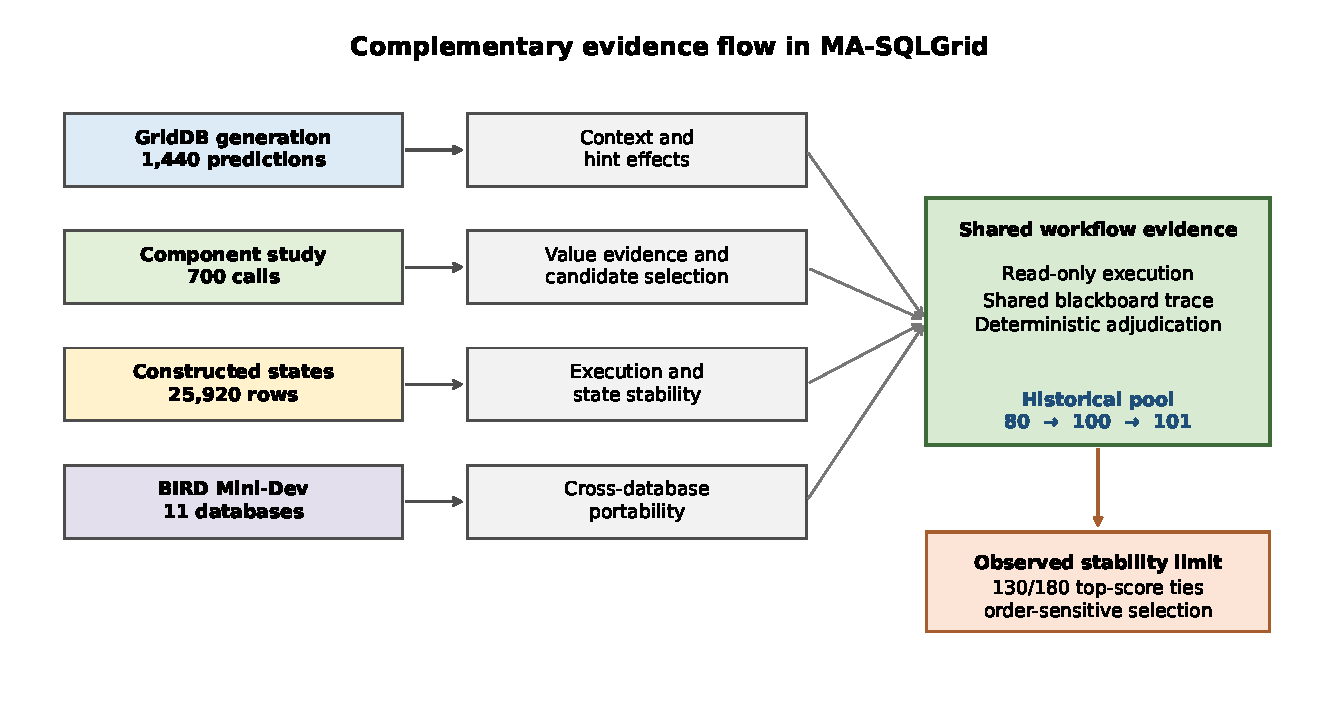
\includegraphics[width=0.88\textwidth]{figures/fig06_evidence_map.pdf}
\caption{Evidence flow from generation studies to read-only validation, constructed-state analysis, and historical-pool selection. The four empirical streams answer complementary questions and are not pooled into one framework accuracy.}
\label{fig:evidence-map}
\end{figure}

\section{Limitations and Future Work}

\textbf{Data and external validity.} GridDB is a synthetic database with eight tables, 98 rows, and 180 evaluation questions, and its evaluation partition was visible during development. BIRD broadens database coverage but is not a grid benchmark. RTS-GMLC, SimBench, and NERC-derived question--SQL assets remain machine-adjudicated silver resources. The next evaluation should use unseen grid schemas and queries independently reviewed by power-system and database specialists for projections, units, time semantics, ordering, and tie handling.

\textbf{Experimental design.} The historical candidate pool combines two backbones and four prompt cells whose outcomes had been examined during earlier development. It supports a descriptive selector comparison, not an end-to-end five-role effect. A new study should hold model snapshot, decoding, candidate count, physical calls, token budget, executor, and evaluator constant across a direct single-candidate baseline, staged one-candidate handoffs, validation-aware multi-candidate selection, and the same selection design with registered state evidence.

\textbf{Semantic validity.} Read-only execution and constructed states test admissibility, executability, and selected invariances. They do not establish that a query reflects a grid professional's intended business meaning. Future work should combine expert review with reference-independent evidence for units, status definitions, time windows, topology relations, and result granularity. Model- or author-assisted triage should remain distinct from independent expert adjudication.

\textbf{Ranking stability.} The high tie rate and candidate-order sensitivity show that the current evidence score is weak when several candidates execute successfully. Future protocols should calibrate semantic ranking, abstention margins, and clarification policies on development-only data and report risk--coverage on an untouched evaluation set. A trained schema linker and low-confidence full-schema fallback can be introduced within the same trace interface, with every change receiving a new protocol identity.

\section{Conclusions}

\masql{} reframes power-grid Text-to-SQL as a traceable multi-role decision process. Five specialized roles separate intent analysis, schema mapping, candidate normalization, read-only execution validation, and constructed-state evidence. A deterministic controller records their handoffs through a shared blackboard trace, selects only eligible candidates, and can abstain when required evidence is incomplete. This architecture provides a reproducible interface for locating errors that would be hidden by a final-SQL-only pipeline.

The experiments show that context and value evidence depend on the model and evaluation setting. The clearest selection result arises within the frozen historical pool: fixed order produced 80/180 reference matches, validation-aware ranking produced 100/180, and complete witness evidence produced 101/180. The 20--21-match difference supports validation-aware selection as a promising design direction. At the same time, top-score ties on 130/180 questions and the 117--118/180 reverse-order sensitivity expose an unresolved semantic-ranking problem.

MA-SQLGrid therefore offers a practical foundation for auditable power-grid Text-to-SQL research rather than a completed deployment system. The next step is a call- and budget-matched evaluation on unseen, independently expert-reviewed grid queries, with pre-registered semantic evidence, tie handling, abstention, and risk--coverage analysis.

\supplementary{The Supplementary Materials contain: Section S1, software conformance and executor tests; Section S2, protocol identities, version chronology, incident disposition, and artifact hashes; Section S3, complete GridDB, component, constructed-state, BIRD, replay, tie, order-sensitivity, and Q039 numerical tables; Section S4, figure lineage, rights inventory, and reproducibility instructions; and Section S5, reviewer verification and release checks. The package excludes credentials, caches, restricted third-party source records, and superseded or incident outputs presented as scientific results.}
\authorcontributions{Conceptualization, B.L. and Y.Y.; methodology, B.L.; software, B.L.; validation, B.L. and C.S.; formal analysis, B.L. and C.S.; investigation, B.L. and C.S.; resources, Y.Y.; data curation, B.L. and C.S.; writing---original draft preparation, B.L.; writing---review and editing, C.S. and Y.Y.; visualization, B.L.; supervision, Y.Y.; project administration, Y.Y.; funding acquisition, Y.Y. All authors have read and agreed to the published version of the manuscript.}
\funding{This research was funded by the Science and Technology Research Project of State Grid Fujian Electric Power Co., Ltd., grant number 521300250006. The funder had no role in the study design; in the collection, analysis, or interpretation of data; in the writing of the manuscript; or in the decision to publish the results.}
\institutionalreview{Not applicable. This study did not involve human participants or animals.}
\informedconsent{Not applicable.}
\dataavailability{The implementation repository is available at \url{https://github.com/gaoxingkele/ma-sqlgrid}, and BIRD Mini-Dev remains available from its public provider. The manuscript-bound rights-safe verification package, including the numerical supplement, code, tests, rights inventory, supersession notice, and independent audits, is available from the corresponding author upon reasonable request. Owing to third-party licensing restrictions, restricted source records and source-dependent RTS-GMLC or SimBench artifacts may be shared for editorial and peer-review verification only when permitted by the applicable third-party licenses. Reviewer access does not constitute a redistribution license.}
\acknowledgments{During reconstruction and revision of this manuscript, the authors used the OpenAI Codex agent interface for prose drafting and editing, experimental and audit suggestions, Python/\LaTeX{} code review and drafting, provenance assembly, reproducibility checks, and local build/visual-quality assistance. The exact backend model identifier/version was not retained in the project records; no unrecorded identifier is inferred. All reported values were obtained from retained executable ledgers and local analyses; Codex output was not treated as qualified expert annotation or independent scientific adjudication. All six scientific figures are code-native and no generative-image output is used as quantitative evidence. The authors reviewed and edited the outputs and take full responsibility for the publication.}
\conflictsofinterest{The authors declare no conflicts of interest.}

\begin{adjustwidth}{-\extralength}{0cm}
\reftitle{References}
\bibliography{references_verified}
\PublishersNote{}
\end{adjustwidth}
\end{document}
